Javaに親しい読者はideaに詳しいことでしょう。ideaはプラグインを通してgo言語のシンタックスハイライト、コード補完およびリビルドをサポートしています。

\begin{enumerate}
  \item ideaを先にダウンロードします。ideaはマルチプラットフォームをサポートしています:win,mac,linux、もしお金があれば正式版を購入します、もし無ければ、コミュニティの無料版を使ってください。Go言語を開発するだけであれば無料版で十分事足ります。
    \begin{figure}[H]
      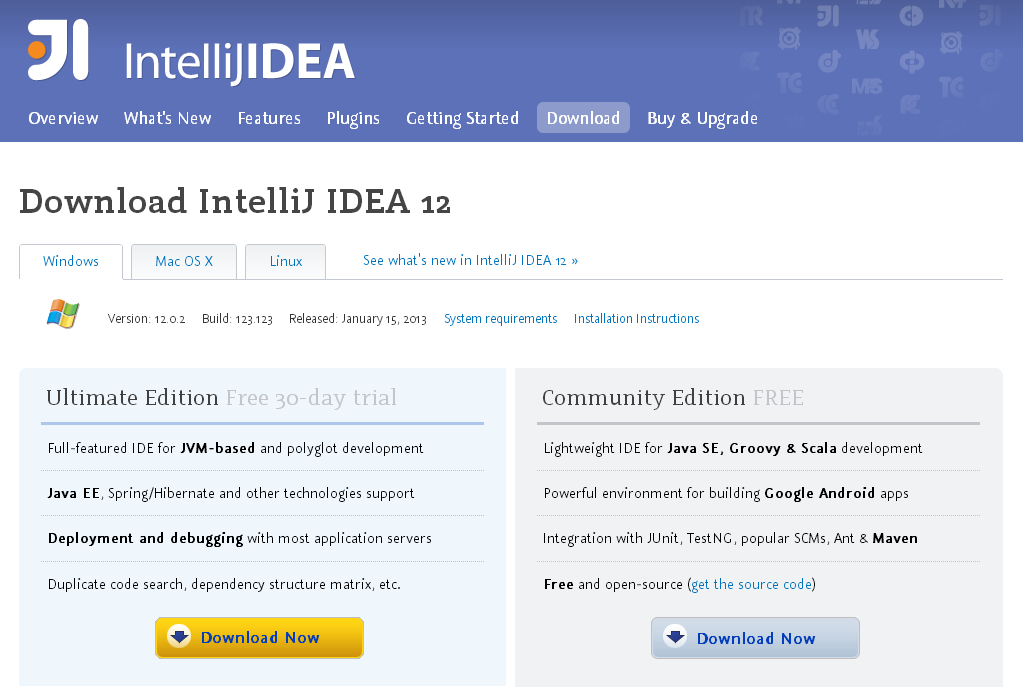
\includegraphics[width=14cm]{1.4.idea1.png}
    \end{figure}
  \item Goプラグインをインストールし、FileメニューのSettingをクリックします。Pluginsを探したら、Browser repoボタンをクリックします。中国国内のユーザはおそらくエラーが出るかもしれませんが、自分で解決してくれよな。
    \begin{figure}[H]
      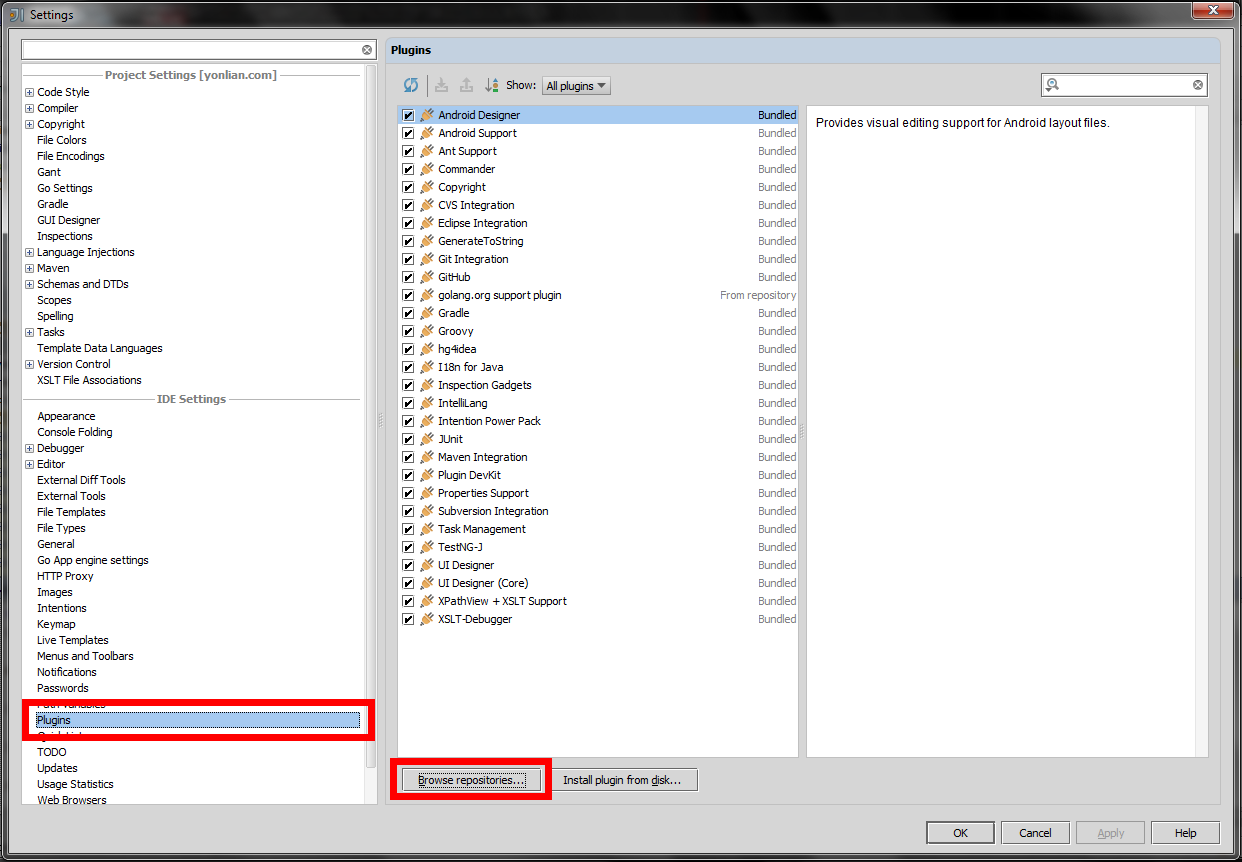
\includegraphics[width=14cm]{1.4.idea3.png}
    \end{figure}
  \item この時いくつものプラグインが見つかります。Golangを検索して、download and installをダブルクリックしてください。golangの行末にDownloadedの表示が現れるのを待って、OKをクリックします。
    \begin{figure}[H]
      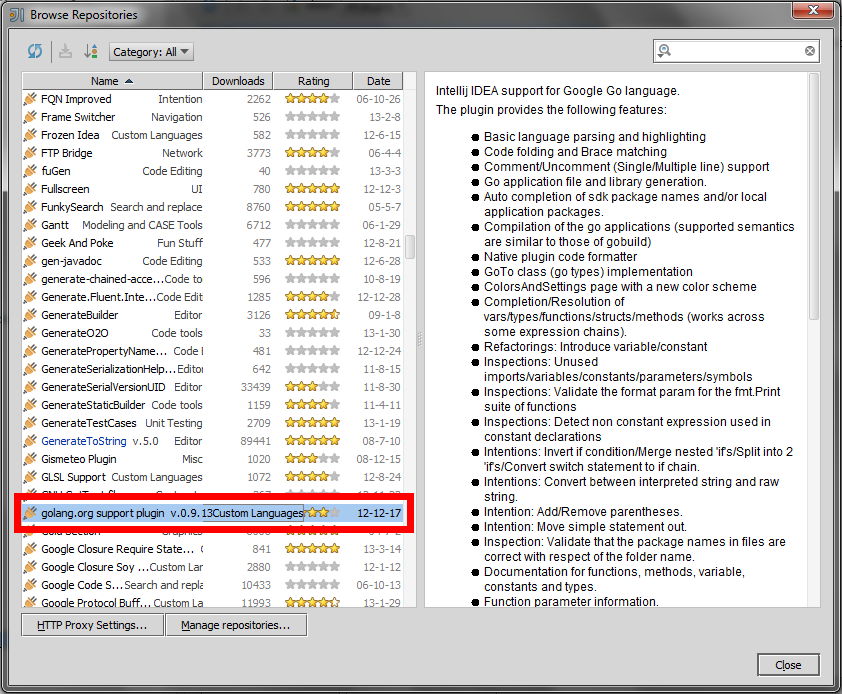
\includegraphics[width=14cm]{1.4.idea4.png}
    \end{figure}
    その後Applyをクリックすると、IDEが再起動を要求します。
  \item 再起動が完了し、新規プロジェクトを作成すると、golangプロジェクトが作成可能であることがお分かりいただけるかとおもいます:
    \begin{figure}[H]
      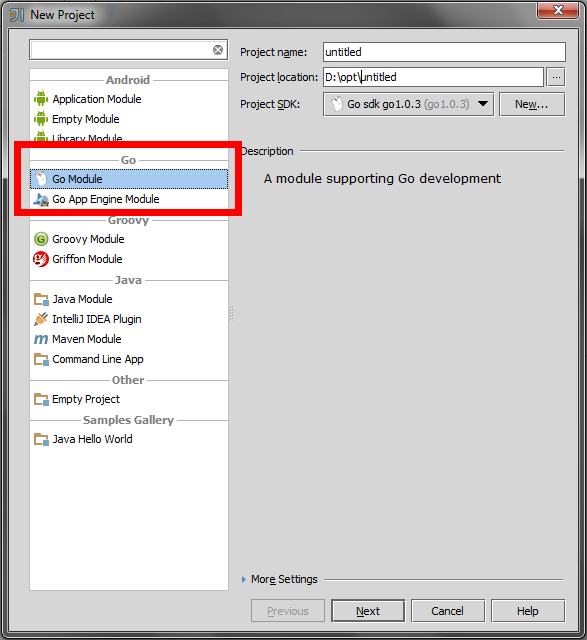
\includegraphics[width=14cm]{1.4.idea5.png}
    \end{figure}
    次に、go sdkの場所を入力するよう促されるかもしれません。普段はいつもC:\textbackslash Goにインストールされています。Linuxとmacは自分のインストールディレクトリの設定にしたがって、ディレクトリを選択すれば大丈夫です。
\end{enumerate}
